\section{Proposed Method}
\label{sec:method}

\begin{figure*}[t]
  \centering
  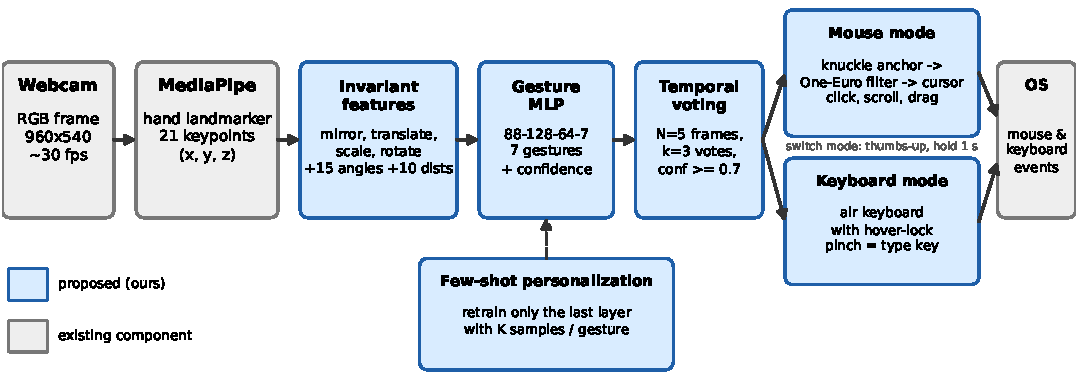
\includegraphics[width=\textwidth]{figures/overview.pdf}
  \caption{\textbf{Overview of our system.} Grey boxes are existing tools and
  blue boxes are our work. Each webcam frame gives 21 hand points. We clean
  them into 88 features, the Gesture MLP names the gesture, and voting makes
  the decision stable. The stable gesture then drives either the mouse
  (knuckle anchor and One-Euro filter) or the air keyboard (hover-lock). A new
  user can personalise the MLP with a few samples.}
  \label{fig:overview}
\end{figure*}

\Cref{fig:overview} shows the whole journey of one camera frame. In this
section we follow that frame from left to right. For each step we say what it
does and why we need it.

\subsection{Step 1: finding the hand}
The webcam gives a $960\times540$ colour frame about 30 times per second. We
flip it like a mirror, so that moving the hand to the right moves the cursor to
the right. MediaPipe's Hand Landmarker~\cite{zhang2020mediapipe} then returns
21 points $\mathbf{p}_i=(x_i,y_i,z_i)$ on the hand and tells us whether it is a
left or a right hand. Point 0 is the wrist, point 4 the thumb tip, point 5 the
index knuckle and point 8 the index tip. \emph{Why:} MediaPipe is accurate,
runs on a CPU and tracks the hand between frames, so most of our time budget
is left for the next steps.

\subsection{Step 2: cleaning the hand points}
\label{sec:features}
The same gesture can give very different raw numbers. The hand may be on the
left or the right of the image, near or far from the camera, tilted, or it may
be a left hand. A classifier would have to learn all these cases from data,
and our dataset is small. So we remove them by geometry
(\cref{fig:features}):
\begin{enumerate}
\item \textbf{Mirror} a left hand, $x_i \leftarrow 1-x_i$, so that one model
works for both hands.
\item \textbf{Move} the wrist to the origin: $\mathbf{q}_i=\mathbf{p}_i-\mathbf{p}_0$.
\item \textbf{Scale} by the palm size, the distance from the wrist to the
middle-finger knuckle: $\mathbf{q}_i \leftarrow \mathbf{q}_i/\lVert(\mathbf{p}_9-\mathbf{p}_0)_{xy}\rVert$.
\item \textbf{Rotate} the points so that the palm always points straight up.
\end{enumerate}
After this, a pointing hand looks the same wherever it is in the image. We
then add 15 bend angles (three joints per finger) and the 10 distances between
every pair of fingertips. These describe the hand shape directly: a pinch is
simply a small thumb-to-index distance. This gives $63+15+10=88$ numbers per
frame.

\begin{figure}[t]
  \centering
  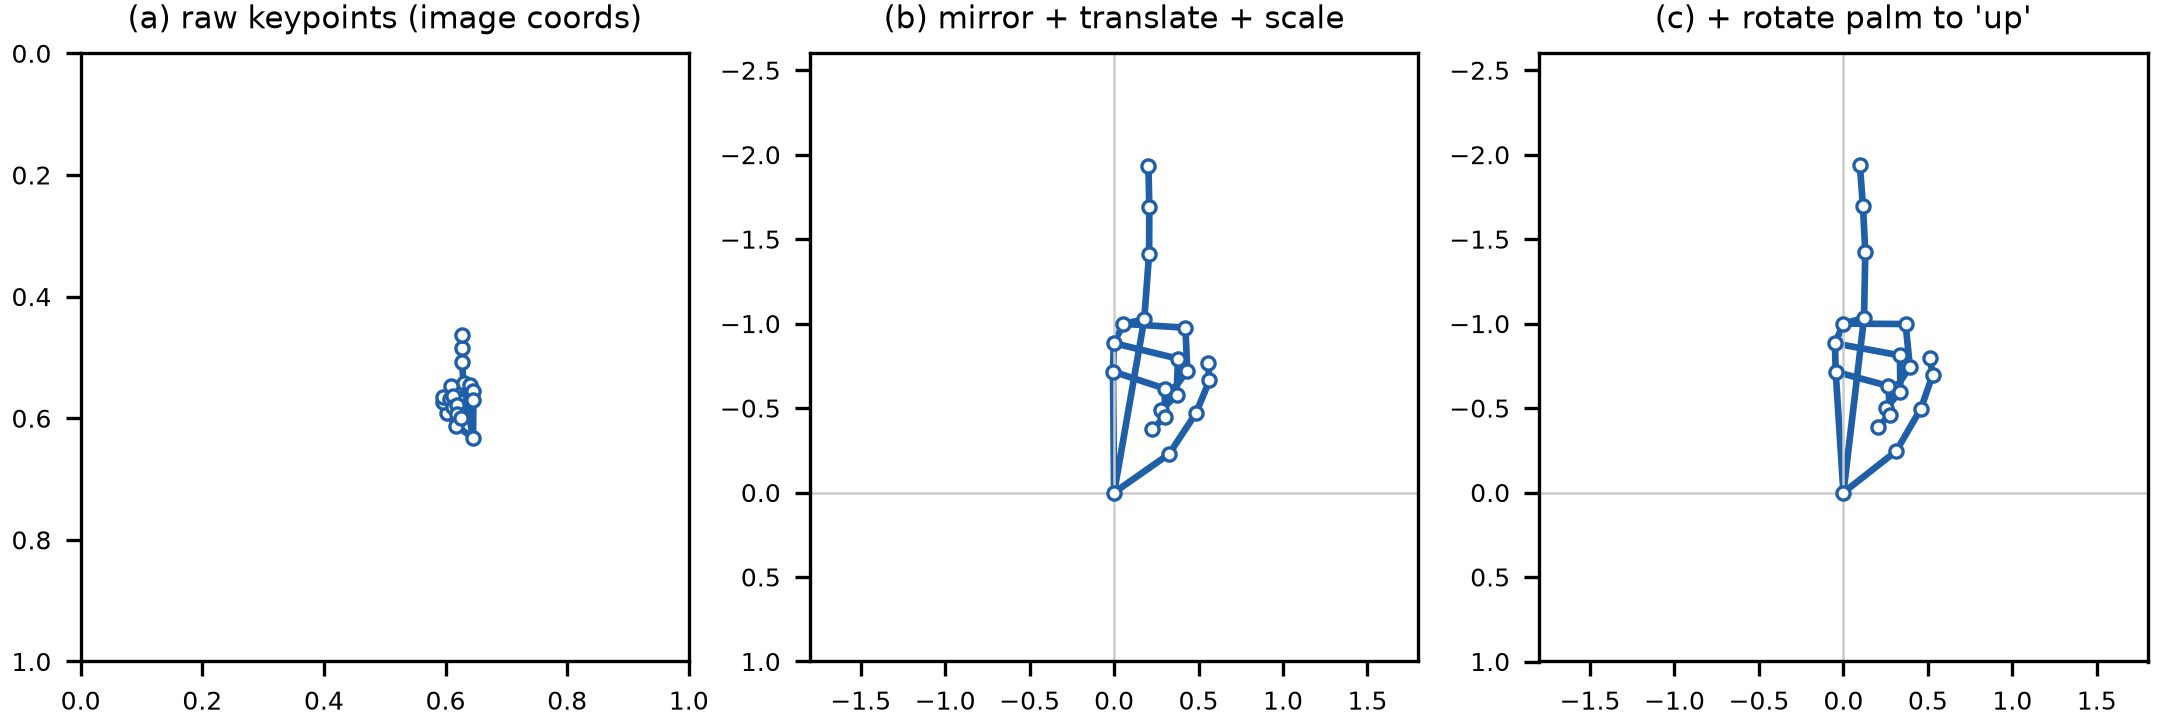
\includegraphics[width=\linewidth]{figures/features.png}
  \caption{\textbf{Cleaning the hand points} for one recorded frame: raw points
  in the image (a), after mirroring, moving and scaling (b), and after
  rotating the palm to point up (c).}
  \label{fig:features}
\end{figure}

\subsection{Step 3: naming the gesture with a neural network}
\label{sec:mlp}
We use 7 gestures (\cref{fig:gestures}). A small multi-layer perceptron (MLP)
reads the 88 features and outputs a probability for each gesture. Its layers
are $88\rightarrow128\rightarrow64\rightarrow7$, with batch
normalisation~\cite{ioffe2015batch}, ReLU and dropout~\cite{srivastava2014dropout}.
It has about 20\,k weights. To make it work for people who are not in the
training data, we show it four extra copies of every training frame. Each copy
is slightly rotated (up to $\pm20^\circ$), scaled (0.85 to 1.15), shifted and
given a little noise (data augmentation).

\emph{Why an MLP and not a CNN on the image?} After Step 2 the input is only 88
numbers, so a tiny network is enough. It runs in under a millisecond on a
CPU, and it never sees the background or the lighting. We check this choice
against an image CNN in \cref{sec:exp-cls}.

\begin{figure}[t]
  \centering
  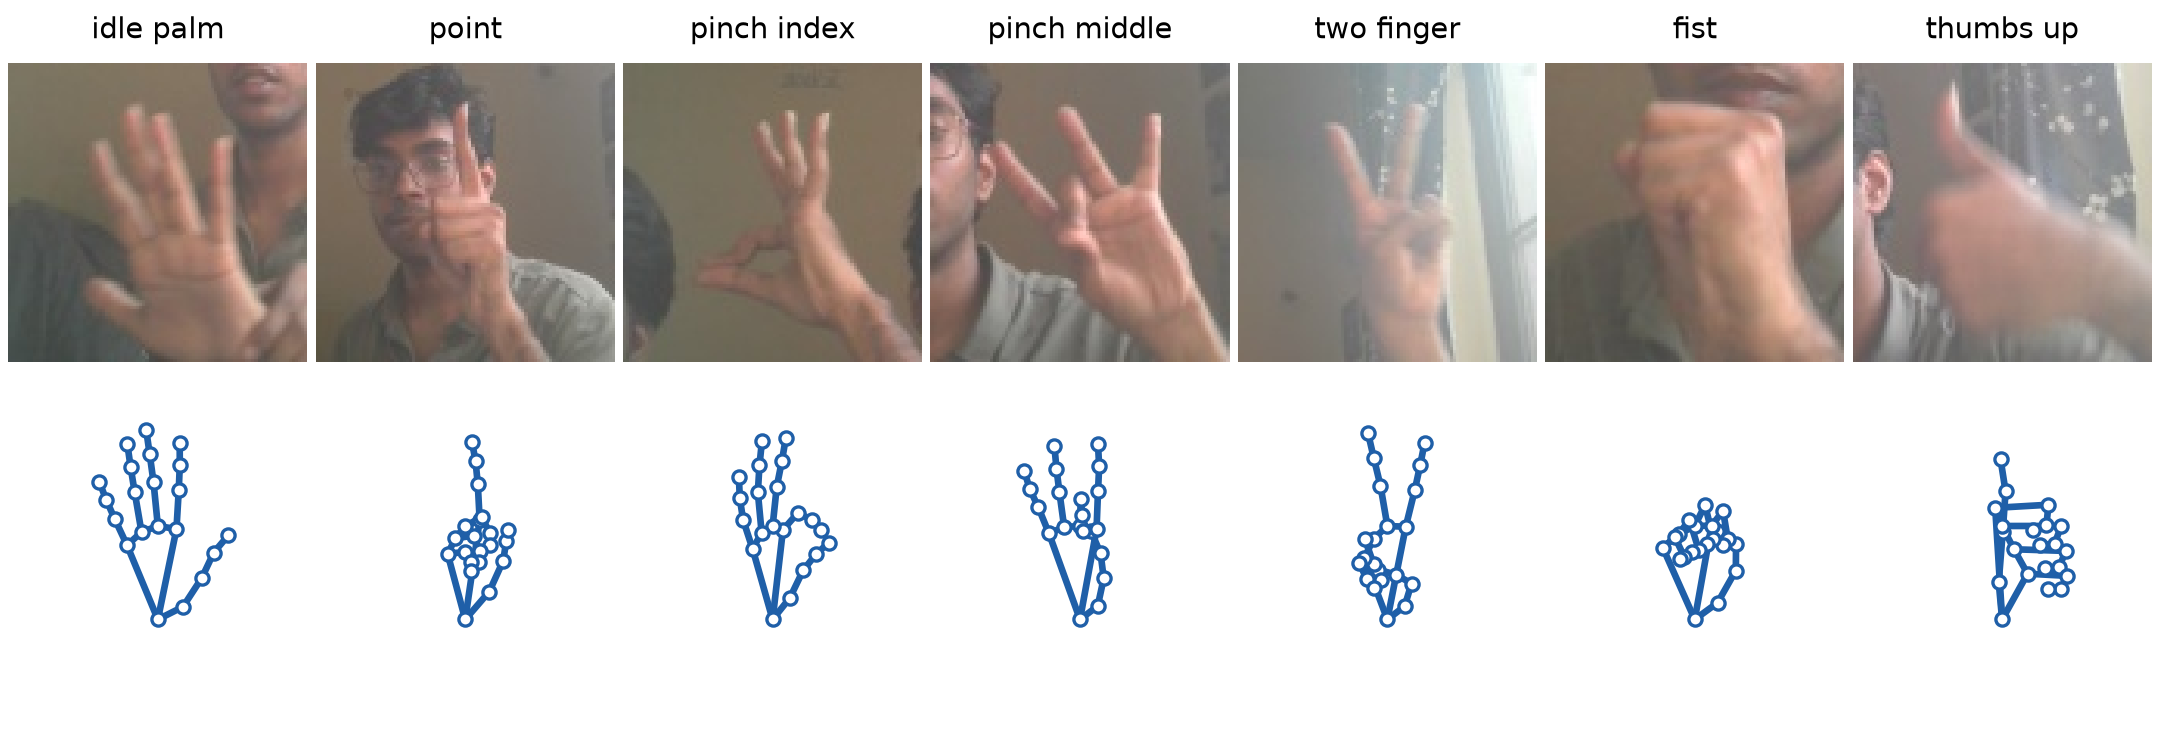
\includegraphics[width=\linewidth]{figures/gestures.png}
  \caption{\textbf{Our 7 gestures.} Top: a frame from our dataset. Bottom: the
  typical cleaned hand points of that gesture.}
  \label{fig:gestures}
\end{figure}

\subsection{Step 4: voting over time}
\label{sec:voting}
When the hand moves from ``point'' to ``pinch'', the network can be unsure for
a frame or two. If we acted on every frame, these short mistakes would become
clicks. So we keep the last $N=5$ predictions and their confidences, and we
change the \emph{stable} gesture only when one gesture gets at least $k=3$ of
the 5 votes \emph{and} its average confidence is at least 0.7. Otherwise the
old gesture stays. Actions happen only at the moment a stable gesture
\emph{starts}, with at least 0.35\,s between two clicks. The cost is a delay of
2--3 frames, which is below 100\,ms.

\subsection{Step 5: a steady cursor}
\label{sec:cursor}
\paragraph{Which point should the cursor follow?} Most virtual mice use the
index fingertip. But a click is a pinch, and a pinch moves the fingertip
towards the thumb. Because of the voting delay, the cursor follows that moving
fingertip for a few frames before the click happens, so the click lands next to
the target. We use the index \textbf{knuckle} (point 5) instead. It sits under
the pointing finger, so pointing still feels natural, but it hardly moves
during a pinch (\cref{fig:anchor}).

\paragraph{From hand to screen.} A box in the middle of the camera view (the
``active area'') is stretched to fill the whole screen. A small hand movement
can therefore reach every corner.

\paragraph{Smoothing with the One-Euro filter.} Even a still hand gives
slightly different points in every frame. A plain moving average removes this
shake but makes the cursor lag behind the hand. The One-Euro
filter~\cite{casiez2012oneeuro} is a low-pass filter whose cut-off frequency
grows with the hand's speed:
\begin{equation}
  \hat X_t = \alpha_t X_t + (1-\alpha_t)\,\hat X_{t-1},\quad
  \alpha_t = \frac{1}{1+\frac{1}{2\pi f_c\,\Delta t}},\quad
  f_c = f_{\min} + \beta\,|\dot{X}_t| .
\end{equation}
When the hand is slow, $f_c$ is low and the shake is removed. When the hand is
fast, $f_c$ is high and there is no lag. We use $f_{\min}=1$\,Hz and
$\beta=0.02$ on screen pixels.

\begin{figure}[t]
  \centering
  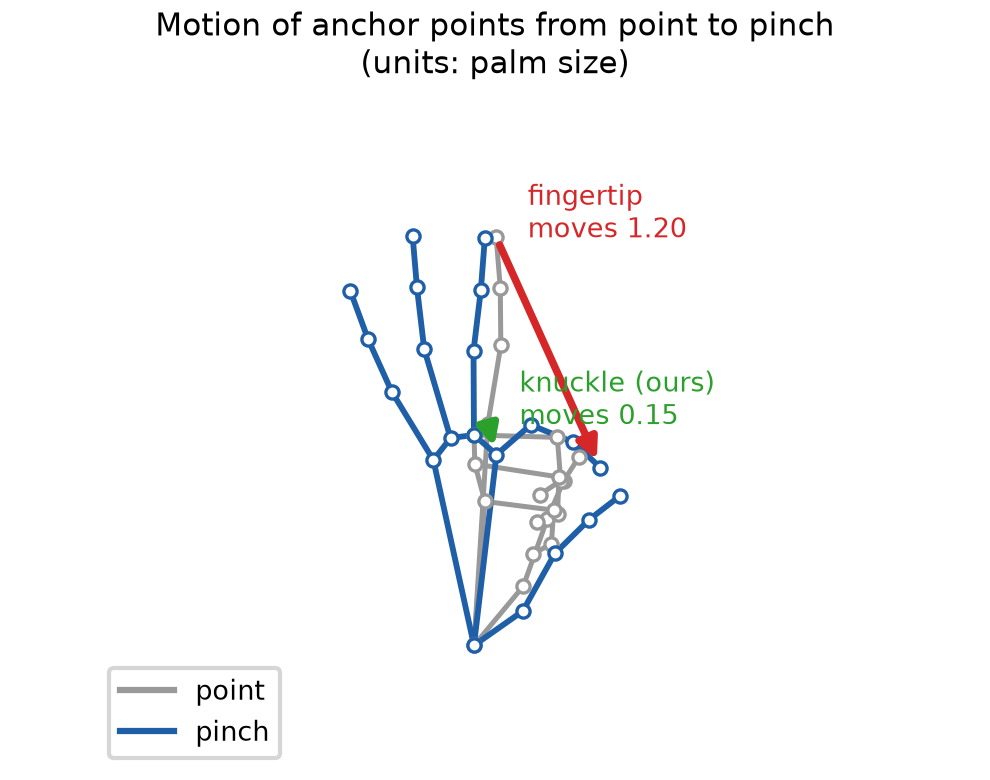
\includegraphics[width=0.85\linewidth]{figures/anchor.png}
  \caption{\textbf{Why we use the knuckle.} A typical ``point'' hand (grey) and
  ``pinch'' hand (blue) from our data, placed on the same wrist. When the user
  pinches, the fingertip moves much more than the knuckle.}
  \label{fig:anchor}
\end{figure}

\subsection{Step 6: actions and the air keyboard}
\label{sec:actions}
\Cref{tab:gestures} lists what each stable gesture does. Actions are sent to
the operating system with PyAutoGUI~\cite{pyautogui}. Holding a thumbs-up for
one second switches to keyboard mode. A QWERTY keyboard is then drawn on the
camera view, and the key under the index fingertip is highlighted. A pinch
types it. Here the pinch again moves the fingertip, by about one key, so we
add a \textbf{hover-lock}: we type the key that was highlighted in the last
``point'' frame \emph{before} the pinch.

\begin{table}[t]
  \centering\small
  \caption{Gestures and what they do.}
  \label{tab:gestures}
  \begin{tabular}{@{}lll@{}}
    \toprule
    Gesture & Mouse mode & Keyboard mode \\
    \midrule
    Open palm & pause (cursor stays) & -- \\
    Point (index up) & move cursor & highlight key \\
    Pinch thumb + index & left / double click & type key \\
    Pinch thumb + middle & right click & -- \\
    Two fingers up (V) & scroll & -- \\
    Fist & drag & -- \\
    Thumbs up, 1\,s & to keyboard mode & to mouse mode \\
    \bottomrule
  \end{tabular}
\end{table}

\subsection{Step 7: one-second personalization}
\label{sec:personal}
Every person makes gestures a little differently. Early layers of a network
learn general features, and the last layer is the most task-specific
one~\cite{yosinski2014transferable}. So for a new user we freeze the network and
re-train only its last layer (455 weights) on $K$ samples per gesture from that
user. This takes about one second on a CPU and can be done just before use.
